\section{Data Augmentation}
\subsection{Data augmentation methods}
There are few different ways how to deal with class imbalance using augmentation \cite{bloem2020methology1}. Horizontal and vertical shifting, zooming, tilting and vertical flipping (mirroring) is used to augment the underrepresented classes. This is achieved with the "ImageDataGenerator" function from the Keras framework \cite{imagepreprocessing-kerasdocumentation}. \\


\subsection{Method}
The data is augmented using the "ImageDataGenerator" function from Keras for each class. ImageDataGenerator has multiple parameters which influence the augmentation of images. Width-shift range, height-shift range, rotation-range, zoom-range and vertical-flip are used. Height-shift and width-shift range "shift" the images in a given range of for example 10 pixels in height, width or combined. Rotation-range "rotates" an image by a certain degree given in the set range. Zoom-range "zooms" an image by a given percentage. Vertical-flip "mirrors" the image.\\
The amount of the to be generated images is determined by a function that detects the most occurring class, counts the images available for this class and creates augmented images for the underrepresented classes to match the amount of images of the most occurred class. After the creation of the augmented images, the images are merged with a copy of the original training set. This results in a new data set without class imbalance with variations of the augmented images set in the "ImageDataGenerator" function.\\
Each parameter was tested individually with different values and in every possible combination with the other parameters. This resulted in 164 different combinations. Due to limited hard drive capacity, cloud storage capacity (the augmented data was 55GB big) and training time, more combinations could not be tested. \\
The width- and height-shift were both tested with a shift range of 0, 5 and 10.\\
The zoom-range was tested with a percentage of 0, 10 and 20. \\
The rotation-range was tested with 0,10 and 20 degrees. \\
Vertical-flip was tested with the values 0 for off and 1 for on.\\

\subsection{Initial results on validation set}
Initially, the train and validation set was created each time the CNN was trained instead of splitting the dataset (excluding the test set) into the train and validation set once. This meant that augmented data was in both the training and validation set.\\
This lead to the phenomena that the results would not differ from the training baseline when taking into consideration some randomness. Even when shifting the images by up to 224 pixels (the whole width or height) the results would not differ. Figure \ref{fig:shift_img} is an example of such an extreme augmentation but not the most extreme, some pictures were just black.
\begin{figure}[h]
    \centering
    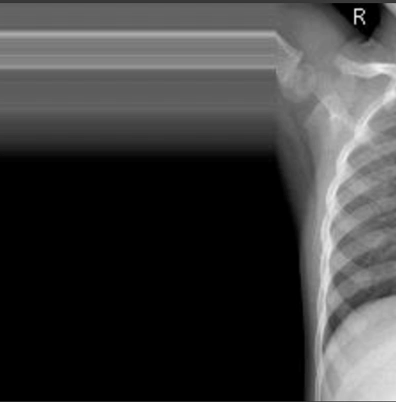
\includegraphics[width=0.4\linewidth]{figures/augmentation/faulty_image_example.png} 
    \caption{Notable Shifting of Image}
    \label{fig:shift_img}
\end{figure}
This should not yield the same results as the training baseline, but initially it did. The problem was likely the split at the beginning of each training. The "faulty" augmented data was present in both the train and validation set. Our design decision to create a train and validation set each for each training introduced errors to the validation set which would have likely resulted in devastating results on the test set.

\subsection{Results on Validation Set} 
To correct the introduction of faulty data into the validation set, the train and validation set split was changed to happen only once.\\
Surprisingly, even this corrected method did not show substantial differences from the training baseline, which would allow for a confident conclusion that this data augmentation method does indeed result in better results and the different results are not just due to some randomness. \\
All 164 results yield results in both precision and recall in a similar range as the training baseline. Which can be seen in figure \ref{fig:augm_val}.

\begin{figure}[!ht]
    \centering
    \subfloat[Precision]{\label{fig:augm_val_a}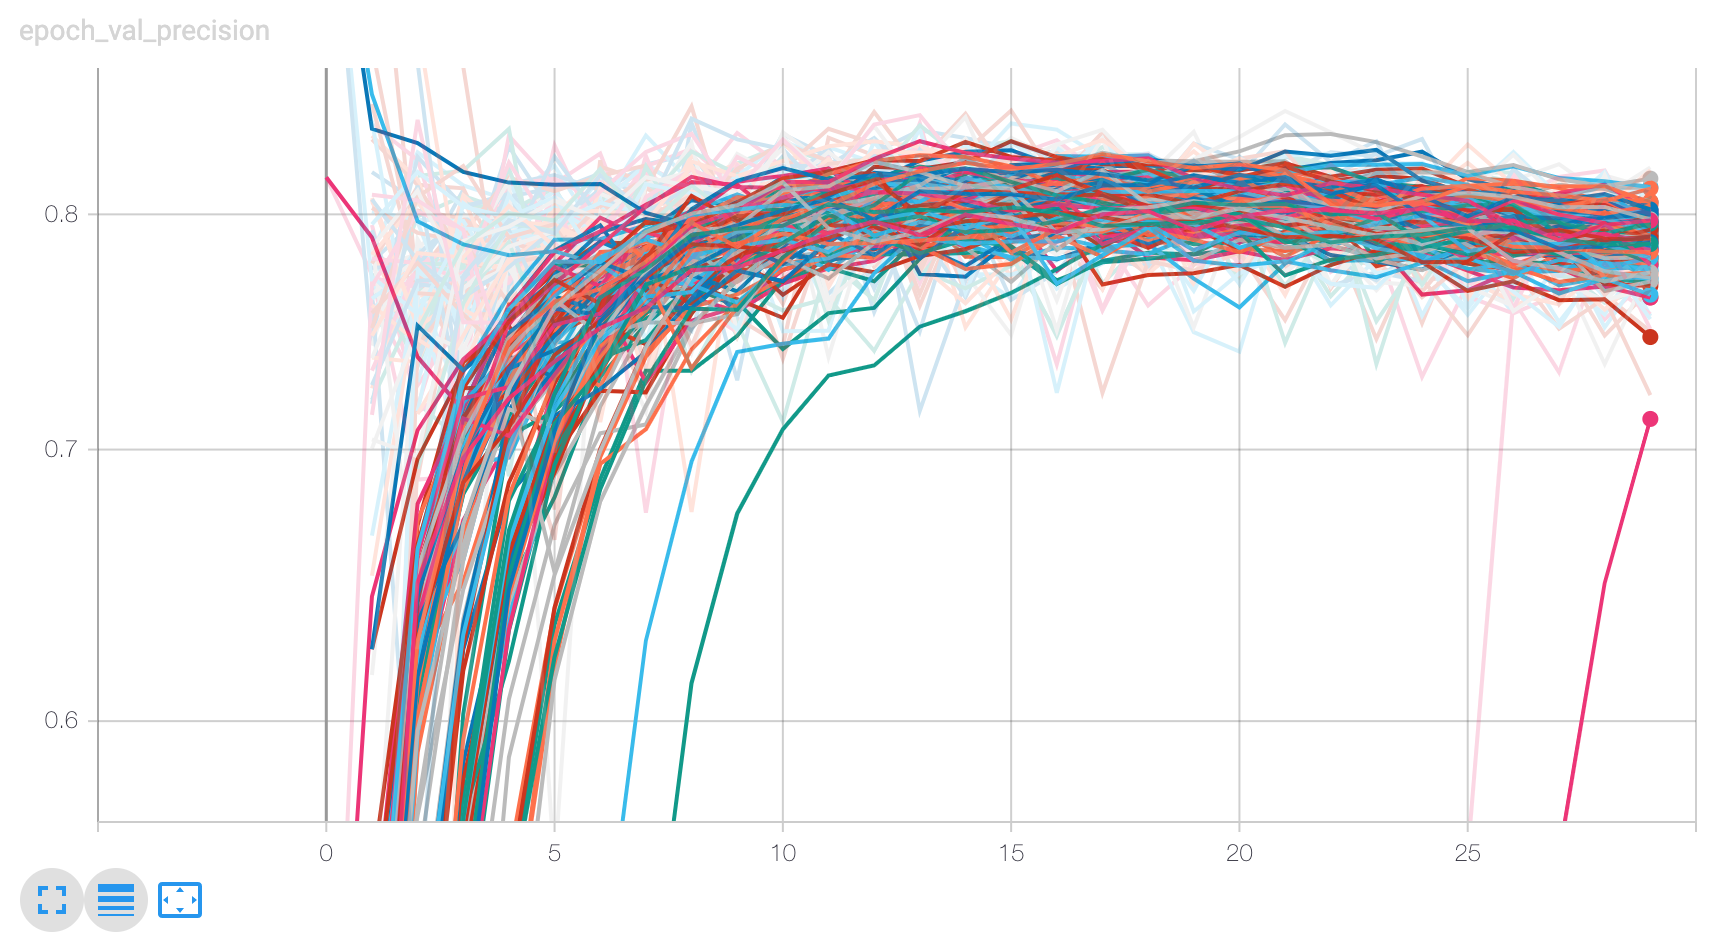
\includegraphics[width=0.89\linewidth]{figures/augmentation/val_precision.png}}
    \par\medskip
    \centering
    \subfloat[Recall]{\label{fig:augm_val_b}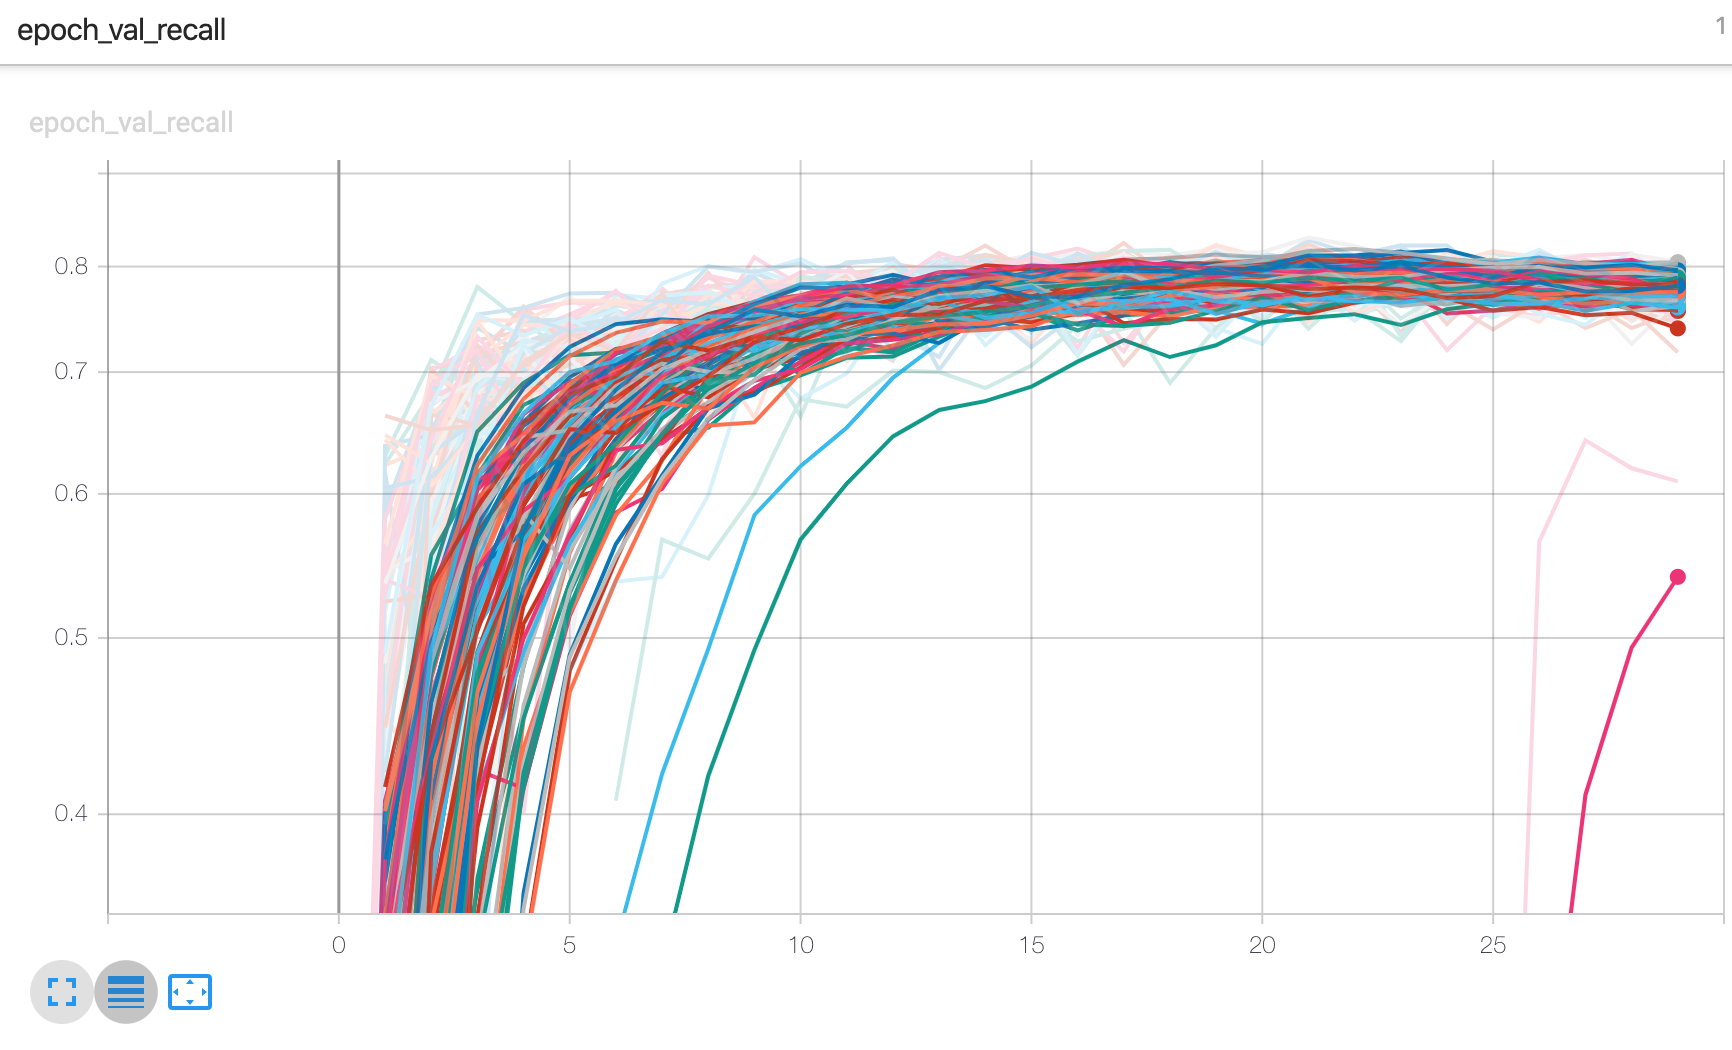
\includegraphics[width=0.89\linewidth]{figures/augmentation/val_recall.png}}
    \par\medskip
  \caption{Augmentation on Validation Set with 164 different combinations. The range of all results are close which indicates no clearly better combination(s) or method(s).}
  \label{fig:augm_val}
\end{figure}

\subsection{Results on Test Set}
Unfortunately, the scalar (graphs) can not be exported from TensorBoard for further analysis. We suspect this might be due to the resulting data size. Due to these limitation, or because these augmentation methods seem to not make a difference, each parameter is validated on the test individually with the "middle" value. E.g. width-shift was tested with a range of 0, 10 and 20. Therefore, the "middle" value for width-shift is 10. The only exception is vertical-flip since this is a Boolean value. This value is tested with 1 for true. The results are shown in the following table:

\begin{table}[h]
\centering
\begin{tabular}{ |p{3cm}|c|c|  }
 \hline
 \multicolumn{3}{|c|}{Augmentation results on test set} \\
 \hline
 Method & Precision & Recall\\
 \hline
 Baseline & 0.7019 & 0.7087\\
 Vertical-flip(1) & 0.6981 & 0.6891\\
 Rotation-range(10) & 0.6418 & 0.6346\\
 Zoom-range(10) & 0.7325 & 0.7196\\
 Height-shift(10) & 0.7047 & 0.6923\\
 Width-shift(10) & 0.6765 & 0.6635\\
 \hline
\end{tabular}
\end{table}

The vertical-flip and height-shift are close to the baseline results while the results for rotation-range and width-shift are lower. Only the results of zoom-range are higher than the baseline especially for the precision metric. However, it should be noted that these results likely have limited implication due to their ambiguity. No augmentation method seems to clearly outperform the baseline or clearly underperform. Rotation-range and width-shift seem to indicate worse performance but a confident conclusion that this indeed the case can not be made. Although zoom-range seem to perform better, the results are so close to the baseline that no confident conclusion can be drawn either. \\
It can be speculated that rotation of images does indeed lead to worse performance since an x-ray is more or less "straight" most of the times. This could lead to "irritating" patterns when the convolutional layers are generated. Theoretically, zoom-range would sustain the general pattern which may explain the seemingly better performance.






